\documentclass[11pt,a4paper]{article}
\usepackage[margin=1in]{geometry}
\usepackage{hyperref}
\usepackage{enumitem}
\usepackage{xcolor}
\usepackage{listings}
\usepackage{tikz}
\usetikzlibrary{positioning, arrows.meta}

\lstset{
  basicstyle=\ttfamily\small,
  breaklines=true,
  frame=single,
  columns=fullflexible,
}

\title{\bfseries Week 2: Branching Workflow, Google Auth,
  and the Onboarding Flow}
\author{Yash \\ \small Roll No: 1024030846}
\date{4 September 2026}

\begin{document}
\maketitle

\section{Context}
Following on from Week 1's scaffolding and CI/CD pipeline, this
week's work covered three things: putting a real branching
discipline in place, replacing the placeholder authentication
approach with the one actually needed for production, and
designing \emph{and} implementing the first real feature --
new-user onboarding -- using a structured, review-gated
development process.

\section{Branching Workflow}
Set up a proper \texttt{Dev} $\to$ \texttt{feature/*} branching
model on GitHub, since the team will now be working in parallel:

\begin{itemize}[leftmargin=0.7cm]
  \item \texttt{main} -- protected, production, requires a PR
    with at least 1 approval.
  \item \texttt{Dev} -- protected integration branch, requires a
    PR (self-merge allowed for speed), deploys as a Vercel
    \emph{preview}, not production.
  \item \texttt{feature/<name>} -- cut from \texttt{Dev}, one per
    task, PR'd back into \texttt{Dev}.
\end{itemize}
Also updated the CI/CD workflow so pushes to \texttt{Dev} deploy
as preview rather than accidentally matching the old
production-deploy condition, which only checked "is this a pull
request" rather than "is this specifically \texttt{main}".

\section{Database: Prisma Schema for Onboarding}
Added five new fields to the \texttt{Profile} model and two new
enums (\texttt{ComfortLevel}, \texttt{Availability}), migrated
against the real Neon Postgres database set up in Week 1. This
schema supports both onboarding paths described below without
needing a second migration later.

\section{Authentication: From GitHub-as-Login to College Google
  Sign-In}
The original plan (and Week 1's implementation) used GitHub OAuth
as the sign-in method. On review, this was the wrong design: the
platform's actual requirement is that only verified college
students can sign up, and GitHub accounts carry no such guarantee.

\textbf{Redesign:} sign-in is now Google-only, using Auth.js v5,
restricted to a configurable college email domain via a
\texttt{signIn} callback:
\begin{lstlisting}[language=JavaScript]
callbacks: {
  async signIn({ user }) {
    if (!ALLOWED_EMAIL_DOMAIN) return true;
    return Boolean(
      user.email?.endsWith(`@${ALLOWED_EMAIL_DOMAIN}`)
    );
  },
}
\end{lstlisting}
GitHub is no longer part of login at all -- it is deferred to a
later, optional "connect your GitHub" step, used purely as an
evidence source once a student is already signed in.

\subsection{Version choice: Auth.js v5 over the ``latest'' tag}
\texttt{npm install next-auth} resolves \texttt{latest} to a 4.x
release built for the older Pages Router; the App Router
integration works only through a compatibility shim. Pinned
instead to \texttt{next-auth@5.0.0-beta.32} (Auth.js v5) --
despite the "beta" label, this is the version actually designed
for the App Router and is what essentially every current Next.js
tutorial and real project uses.

\section{Feature: New-User Onboarding Flow}
Designed and implemented the first real product feature: after a
student's first Google sign-in, they are routed to a single
\texttt{/onboarding} screen with two paths.

\subsection{Design}
\begin{itemize}[leftmargin=0.7cm]
  \item \textbf{Path A} (has a resume/GitHub): uploads a resume,
    stored in Vercel Blob, creating an \texttt{EvidenceRecord}
    with \texttt{status: "pending\_parse"} for a future parsing
    pipeline. GitHub connection is a visible but disabled
    "coming soon" button for now.
  \item \textbf{Path B} (Explorer/manual): self-reports comfort
    level, interest tags, availability, and optional project
    links, written directly onto \texttt{Profile}.
\end{itemize}
A key design principle from the project spec: self-reported data
(Path B) is \emph{not} treated as evidence -- only Path A creates
an \texttt{EvidenceRecord}. This was written into the design spec
before implementation and verified afterwards against the real
database.

\begin{figure}[h]
\centering
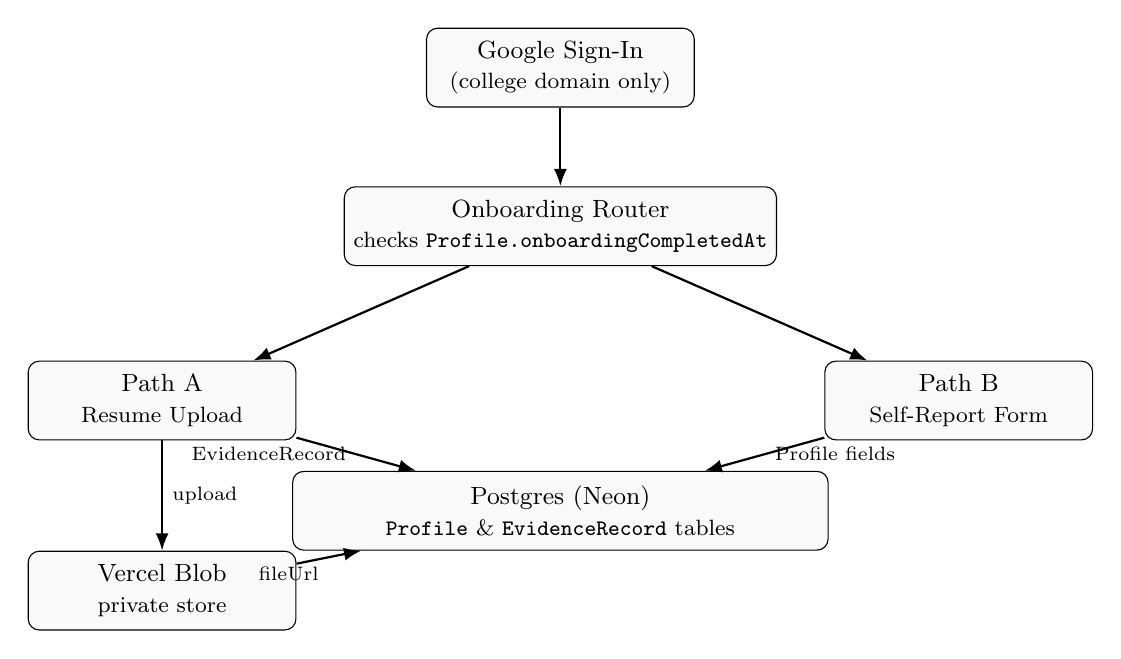
\begin{tikzpicture}[
  node distance=10mm and 10mm,
  box/.style={draw, rounded corners, minimum width=3.4cm,
    minimum height=1cm, align=center, font=\small, fill=gray!5},
  arr/.style={-{Latex[length=2.2mm]}, thick},
  lbl/.style={font=\scriptsize}
]
\node[box] (signin) {Google Sign-In\\\footnotesize(college domain only)};
\node[box, below=of signin] (router)
  {Onboarding Router\\\footnotesize checks
   \texttt{Profile.onboardingCompletedAt}};
\node[box, below left=12mm and 6mm of router] (patha)
  {Path A\\\footnotesize Resume Upload};
\node[box, below right=12mm and 6mm of router] (pathb)
  {Path B\\\footnotesize Self-Report Form};
\node[box, below=14mm of patha] (blob)
  {Vercel Blob\\\footnotesize private store};
\node[box, below=26mm of router, minimum width=6.8cm] (postgres)
  {Postgres (Neon)\\\footnotesize \texttt{Profile} \&
   \texttt{EvidenceRecord} tables};

\draw[arr] (signin) -- (router);
\draw[arr] (router) -- (patha);
\draw[arr] (router) -- (pathb);
\draw[arr] (patha) -- (blob) node[lbl, midway, right] {upload};
\draw[arr] (blob) -- (postgres) node[lbl, midway, below left] {fileUrl};
\draw[arr] (patha) -- (postgres) node[lbl, midway, left] {EvidenceRecord};
\draw[arr] (pathb) -- (postgres) node[lbl, midway, right] {Profile fields};
\end{tikzpicture}
\caption{Onboarding data flow. Path A writes to both Vercel Blob
  and Postgres inside one transaction; Path B writes only to
  Postgres and never touches Blob storage.}
\label{fig:onboarding-flow}
\end{figure}

Route gating was deliberately implemented as a server component
layout (\texttt{app/(protected)/layout.tsx}) rather than
Next.js middleware, because middleware runs on the Edge runtime
by default, and Prisma's client needs the Node runtime -- using
middleware would have required a second, HTTP-based database
driver just for this one check.

\subsection{Process: Design $\to$ Plan $\to$ Subagent-Driven
  Implementation}
Rather than writing the feature directly, followed a structured
process: a written design spec, a detailed implementation plan
broken into 7 tasks with exact interfaces between them, then
execution via a fresh, isolated AI subagent per task, with an
independent review (spec compliance \emph{and} code quality)
after every task, plus one final whole-branch review at the end.
Every task passed its individual review clean or after a small
fix round.

\subsection{Debugging: Public vs.\ Private Blob Storage}
\textbf{Error encountered:} an automated security scan flagged
that resumes (personal, identifying documents) were being stored
with \texttt{access: "public"} on Vercel Blob -- readable by
anyone with the URL, forever.

\textbf{Relevant context:} the original plan specified
\texttt{access: "public"} based on an outdated assumption that
the Vercel Blob SDK only supported public objects.

\textbf{Key observation:} checking the actually-installed SDK
version's type definitions directly
(\texttt{node\_modules/@vercel/blob/dist/index.d.ts}) showed
full support for \texttt{access: "private"}, where the object can
only be read back server-side using the project's own
\texttt{BLOB\_READ\_WRITE\_TOKEN} -- not by anyone with the URL.
This also explained why an earlier upload attempt had failed with
\texttt{Cannot use public access on a private store}: the actual
Blob store was already configured as private, and the code was
wrong, not the store.

\textbf{Solution:} switched \texttt{uploadResume} to
\texttt{access: "private"}. No dashboard changes, no rework --
purely a code correction, and strictly more secure than the
original plan.

\subsection{Debugging: The Vanishing 5MB Resume Limit}
This was the most valuable finding of the week, and it only
surfaced because of the \emph{final}, whole-branch review -- no
single task's isolated review could have seen it, since it lives
in the gap between three different tasks' code.

\textbf{Error (as it would have shown up in production):} a user
uploading a genuinely resume-sized PDF (over 1MB, common once a
resume has any formatting or a headshot) would have the upload
silently rejected by the framework, despite the UI advertising
"max 5MB" and the server code correctly checking for exactly
that limit.

\textbf{Relevant context:} Next.js caps the request body of a
Server Action at 1MB \emph{by default}, independently of any
application-level size check:
\begin{lstlisting}
const nextConfig: NextConfig = {
  /* config options here -- untouched default */
};
\end{lstlisting}

\textbf{Key observation:} the live, manual walkthrough of the
feature used a small test PDF and passed completely -- the bug
was invisible to functional testing precisely because the test
file happened to be under 1MB. It took a reviewer reading the
Next.js documentation shipped inside \texttt{node\_modules}
itself to notice the framework-level cap existed at all.

\textbf{Solution:} raised the limit explicitly in
\texttt{next.config.ts}:
\begin{lstlisting}
experimental: {
  serverActions: {
    bodySizeLimit: "5mb",
  },
},
\end{lstlisting}
Also added a matching client-side size/type check (so a bad file
fails fast, before upload) and wrapped the resume-upload database
transaction in a \texttt{try/catch} so an infrastructure failure
(e.g.\ a Blob outage) returns a clean inline error instead of
crashing the page -- being careful that the \texttt{catch} block
does \emph{not} swallow Next.js's internal redirect mechanism,
which itself works by throwing a special error.

\emph{Because} per-task code review only ever sees one task's
diff at a time, a bug that spans the interaction of three
separate files (UI copy, server validation, and a build config
file none of the three tasks individually touched) can only be
caught by a review that looks at the whole branch at once. This
is the concrete justification for running that final broad
review rather than treating "all tasks passed" as equivalent to
"the feature is correct."

\section{Verification}
No automated test framework exists in this codebase yet, so
verification was manual throughout: TypeScript compiles cleanly,
the production build succeeds, and -- most importantly -- a live
walkthrough against the real Neon database and real Google
accounts confirmed:
\begin{itemize}[leftmargin=0.7cm]
  \item Path A (real PDF upload) correctly creates an
    \texttt{EvidenceRecord} and marks onboarding complete.
  \item Path B correctly populates the self-reported fields and
    creates \emph{no} evidence record.
  \item Revisiting \texttt{/onboarding} after completion redirects
    away.
  \item A signed-out visitor still sees the ordinary sign-in page,
    unaffected by the new gating logic.
\end{itemize}

\section{Outcome}
Opened a pull request into \texttt{Dev} containing the full
onboarding feature, the design spec, and the implementation plan
as project documentation.

\section{Follow-ups}
\begin{itemize}[leftmargin=0.7cm]
  \item Interest tags are currently stored as their display
    labels rather than stable ids -- fine at zero data, worth
    normalising before real usage accumulates.
  \item Resume parsing (turning an uploaded PDF into structured
    skill evidence) is still unbuilt; uploads are stored with a
    \texttt{"pending\_parse"} status for now.
  \item Real GitHub-account linking (as an evidence source, not
    login) remains a separate, not-yet-started piece of work.
\end{itemize}

\end{document}
